\subsection{A boundary integral formulation of electrostatics in molecular solvation}

Figure \ref{fig:implicit_solvent} sketches the continuum representation of a dissolved molecule from the implicit-solvent model. 
In it, the solute is considered as a cavity ($\Omega_1$) inside an infinite medium ($\Omega_2$), and we can compute the change in electrostatic potential as the interior region is charged up with the solute's partial charges, represented as a collection of Direc-delta functions.
The solvent ($\Omega_2$) usually consists of water ($\epsilon_2\approx$80) with salt ions, which are free to move around, forced by the electric field. 
At equilibrium, the salt ions arrange according to a Boltzmann distribution, and if we consider them as point charges, this is well modeled by the linearized Poisson-Boltzmann equation, which considers a screening factor known as the Debye length ($\kappa$.) 
On the other hand, the electrostatics in the solute cavity behaves in agreement with the Poisson equation in a low dielectric medium ($\epsilon_1\approx$2---4), with the solute's point charges as sources.
These two equations are interfaced on the molecular surface ($\Gamma$), where the potential and electric displacement must be continuous.
The resulting system of partial differential equations is
%
\begin{align} \label{eq:pde}
\nabla^2\phi_1 &= \frac{1}{\epsilon_1}\sum_k q_k\delta(\mathbf{r},\mathbf{r}_k) \text{ in the solute ($\Omega_1$),}\nonumber\\
(\nabla^2-\kappa^2)\phi_2 &= 0 \text{ in the solvent ($\Omega_2$),}\nonumber\\
\phi_1 &= \phi_2 \quad \epsilon_1\frac{\partial \phi_1}{\partial\mathbf{n}} = \epsilon_2\frac{\partial \phi_2}{\partial\mathbf{n}} \text{ on the interface ($\Gamma$)}.
\end{align}
%
where $\Omega_1$ and $\Omega_2$ are the solute and solvent regions, respectively, interfaced by the molecular surface $\Gamma$.
There are several available definitions for $\Gamma$, such as van der Waals, solvent accessible (SAS), solvent excluded (SES), and Gaussian surfaces \cite{HarrisFenley2013}, however, in this work we use the SES.
The SES is built by tracking the contact points of a spherical probe of the size of a water molecule ($\sim$ 1.4\AA) as it rolls around the solute atoms (with their corresponding van der Waals radii). 
%
\begin{figure}
\centering
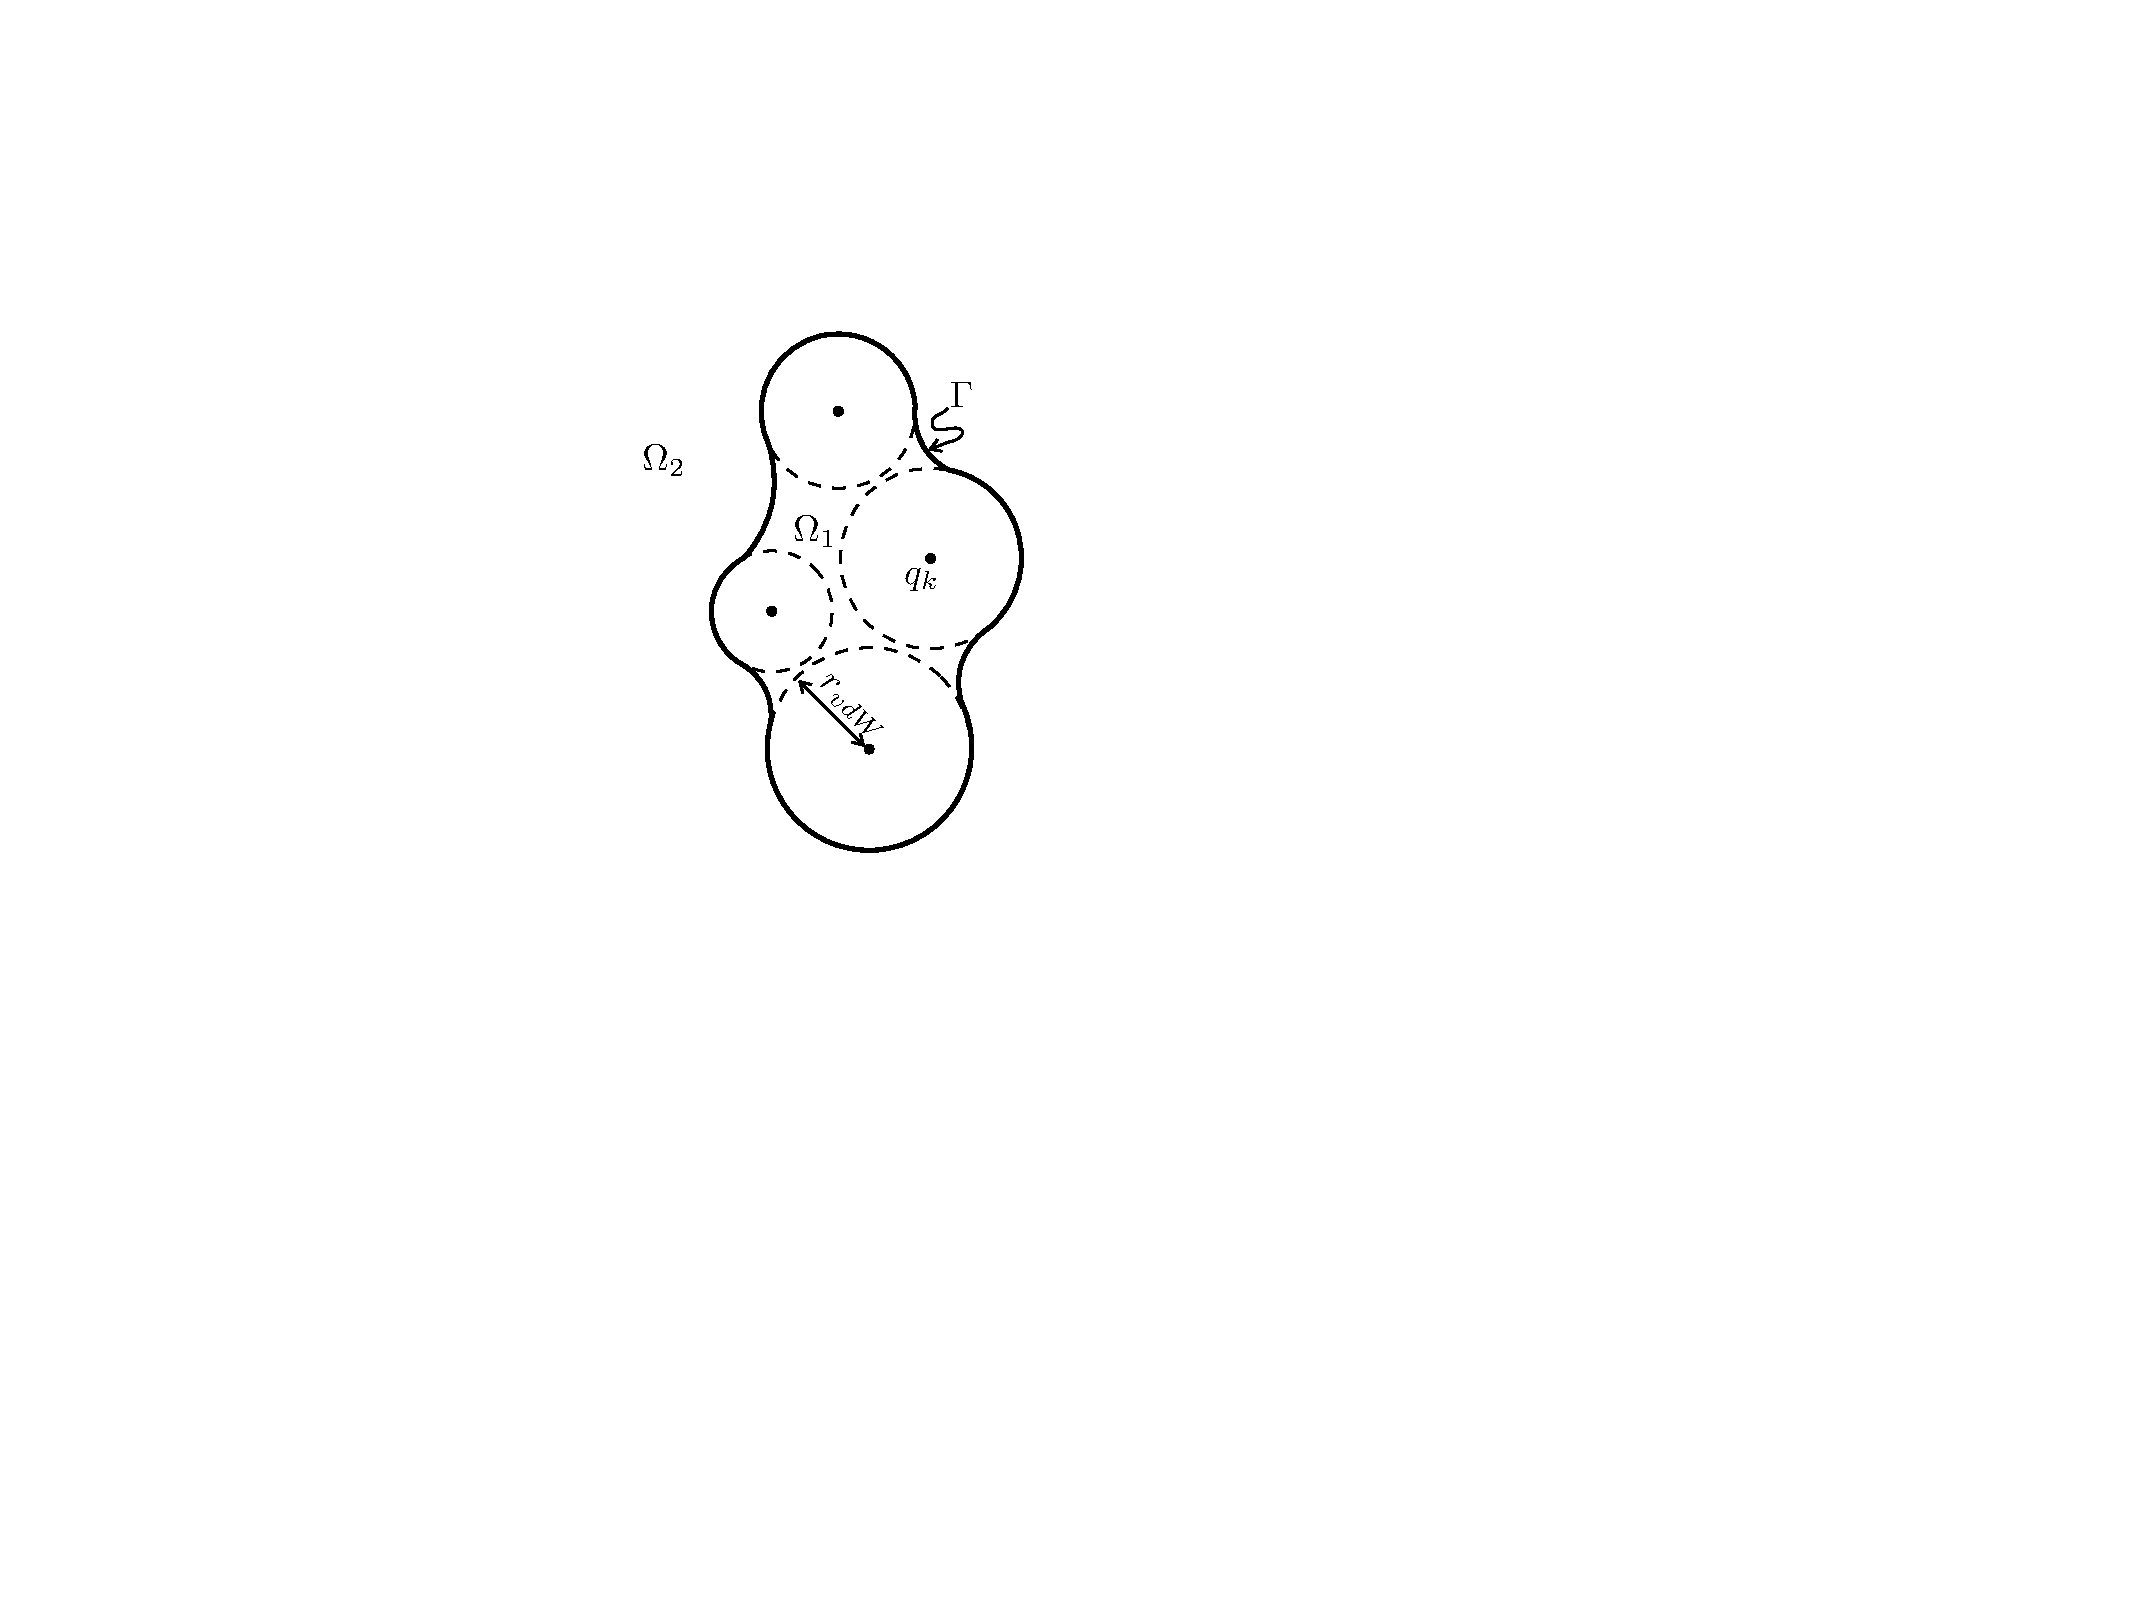
\includegraphics[width=0.25\textwidth]{implicit_solvent.pdf}
\caption{Representation of a dissolved molecule with the implicit-solvent model. The solute ($\Omega_1$) and solvent ($\Omega_2$) regions are interfaced by the solvent-excluded surface ($\Gamma$), and $q_k$ and $r_{vdW}$ are the atomic charge and radii, respectively.}
\label{fig:implicit_solvent}
\end{figure}

Equation \eqref{eq:pde} can be represented as an integral equation running over $\Gamma$ by using Green's second identity, yielding
%
\begin{align} \label{eq:volume_potential}
\phi_{1}+ K_{L}^{\Omega_1}(\phi_{1,\Gamma}) -  V_{L}^{\Omega_1} \left(\frac{\partial}{\partial \mathbf{n}}  \phi_{1,\Gamma}  \right) & = \frac{1}{\epsilon_1} \sum_{k=0}^{N_q}  \frac{q_k}{4\pi|\mathbf{r}_{\Omega_1} - \mathbf{r}_k|}  \quad \text{on $\Omega_1$,} \nonumber \\
\phi_{2} - K_{Y}^{\Omega_2}(\phi_{2,\Gamma}) + V_{Y}^{\Omega_2} \left( \frac{\partial}{\partial \mathbf{n}} \phi_{2,\Gamma} \right) & = 0 \quad \text{on $\Omega_2$,}
\end{align}
%
where $\phi_{1,\Gamma} = \phi_1(\mathbf{r}_\Gamma)$ and $\phi_{2,\Gamma} = \phi_2(\mathbf{r}_\Gamma)$ evaluated at $\Gamma$ approaching from $\Omega_1$ and $\Omega_2$, respectively. $K$ and $V$ are the double- and single-layer potentials for the Laplace (subscript $L$) and modified Helmholtz (Yukawa, subscript $Y$) kernels, which are defined as
%
\begin{align}\label{eq:single_double}
V^\Omega_{L,Y}(\varphi) = \oint_\Gamma G_{L,Y}(\mathbf{r}_\Omega,\mathbf{r}')\varphi(\mathbf{r}')d\mathbf{r}'\nonumber\\
K^\Omega_{L,Y}(\varphi) = \oint_\Gamma \frac{\partial G_{L,Y}}{\partial\mathbf{n}'}(\mathbf{r}_\Omega,\mathbf{r}')\varphi(\mathbf{r}')d\mathbf{r}'\nonumber\\
\end{align}
%
where $\varphi(\mathbf{r})$ is a distribution over $\Gamma$, and $G_L(\mathbf{r},\mathbf{r}')=\frac{1}{4\pi|\mathbf{r}-\mathbf{r}'|}$ and $G_Y(\mathbf{r},\mathbf{r}')=\frac{e^{-\kappa|\mathbf{r}-\mathbf{r}'|}}{4\pi|\mathbf{r}-\mathbf{r}'|}$ are the free space Green's function of the Laplace and linearized Poisson-Boltzmann equations, respectively. 

We can use Equation \eqref{eq:volume_potential} to compute $\phi_\Gamma$ and $\partial\phi_\Gamma/\partial\mathbf{n}$ with either the \emph{direct}~\cite{YoonLenhoff1990} or \emph{derivative}~\cite{JufferETal1991} (also known as \emph{Juffer}) formulations.
The simpler direct formulation is a result of evaluating $\phi_1$ and $\phi_2$ in the limit as $\mathbf{r}$ approaches $\Gamma$, and applying the interface conditions from Equation \eqref{eq:pde}, giving
%
\begin{align} \label{eq:direct}
\frac{\phi_{1,\Gamma}}{2}+ K_{L}^{\Gamma}(\phi_{1,\Gamma}) -  V_{L}^{\Gamma} \left(\frac{\partial}{\partial \mathbf{n}}  \phi_{1,\Gamma}  \right) & = \frac{1}{\epsilon_1} \sum_{k=0}^{N_q}  \frac{q_k}{4\pi|\mathbf{r}_{\Gamma} - \mathbf{r}_k|} \nonumber \\
\frac{\phi_{1,\Gamma}}{2} - K_{Y}^{\Gamma}(\phi_{1,\Gamma}) + \frac{\epsilon_1}{\epsilon_2}V_{Y}^{\Gamma} \left( \frac{\partial}{\partial \mathbf{n}} \phi_{1,\Gamma} \right) & = 0
\end{align}
%
Unfortunately, this formulation is ill-conditioned, as the condition number of the resulting matrix grows unbounded with the number of discretization elements. 
A better conditioned formulation was derived by Juffer \emph{et al.} \cite{JufferETal1992}, where they took the normal derivative of Equation \eqref{eq:potential_volume}, and couple both $\phi$ and $\partial\phi/\partial\mathbf{n}$ on the boundary as follows
%
\begin{align}\label{eq:juffer}
\frac{\phi_{1,\Gamma}}{2}\left(1+\frac{\epsilon_2}{\epsilon_1}\right) - \left(\frac{\epsilon_2}{\epsilon_1}K_Y^\Gamma - K_L^\Gamma\right)(\phi_{1,\Gamma}) &+ \left(V_Y^\Gamma - V_L^\Gamma\right)\left( \frac{\partial}{\partial \mathbf{n}} \phi_{1,\Gamma} \right)\nonumber\\ 
&= \sum_{k=0}^{N_q}  \frac{q_k}{4\pi\epsilon_1|\mathbf{r}_{\Gamma} - \mathbf{r}_k|} \nonumber \\
- \left(W_Y^\Gamma - W_L^\Gamma\right)(\phi_{1,\Gamma}) +  \frac{1}{2}\frac{\phi_{1,\Gamma}}{\partial\mathbf{n}}\left(1+\frac{\epsilon_1}{\epsilon_2}\right) &+ \left(\frac{\epsilon_1}{\epsilon_2}K_Y^{\prime\Gamma} - K_L^{\prime\Gamma}\right)\left( \frac{\partial}{\partial \mathbf{n}} \phi_{1,\Gamma} \right)\nonumber\\ 
&= \sum_{k=0}^{N_q}  \frac{\partial}{\partial\mathbf{n}_\mathbf{r}}\left(\frac{q_k}{4\pi\epsilon_1|\mathbf{r}_{\Gamma} - \mathbf{r}_k|}\right) \nonumber \\
\end{align}
%
Here we use the adjoint double layer ($K'$) and hypersingular ($W$) operators, which are defined as
%
\begin{align}\label{eq:adj_hyp}
K^{\prime\Gamma}_{L,Y}(\varphi) = \oint_\Gamma \frac{G_{L,Y}}{\partial\mathbf{n}}(\mathbf{r}_\Gamma,\mathbf{r}')\varphi(\mathbf{r}')d\mathbf{r}'\nonumber\\
W^\Gamma_{L,Y}(\varphi) = \oint_\Gamma \frac{\partial^2 G_{L,Y}}{\partial\mathbf{n}'\partial\mathbf{n}}(\mathbf{r}_\Gamma,\mathbf{r}')\varphi(\mathbf{r}')d\mathbf{r}'\nonumber\\
\end{align}
%
A slightly modified version of Equation \eqref{eq:juffer} is used in the work from Lu and coworkers~\cite{LuETal2006,LuETal2009,ZhangETal2019}, where they scale the expressions by $\epsilon_1/\epsilon_2$, and solve for the exterior field. This leaves
%
\begin{align}\label{eq:lu}
\frac{\phi_{2,\Gamma}}{2}\left(\frac{\epsilon_1}{\epsilon_2}+1\right) - \left(K_Y^\Gamma - \frac{\epsilon_1}{\epsilon_2}K_L^\Gamma\right)(\phi_{2,\Gamma}) &+ \left(V_Y^\Gamma - V_L^\Gamma\right)\left( \frac{\partial}{\partial \mathbf{n}} \phi_{2,\Gamma} \right)\nonumber\\ 
&= \sum_{k=0}^{N_q}  \frac{q_k}{4\pi\epsilon_2|\mathbf{r}_{\Gamma} - \mathbf{r}_k|} \nonumber \\
- \frac{\epsilon_1}{\epsilon_2}\left(W_Y^\Gamma - W_L^\Gamma\right)(\phi_{2,\Gamma}) +  \frac{1}{2}\frac{\phi_{2,\Gamma}}{\partial\mathbf{n}}\left(1+\frac{\epsilon_1}{\epsilon_2}\right) &+ \left(\frac{\epsilon_1}{\epsilon_2}K_Y^{\prime\Gamma} - K_L^{\prime\Gamma}\right)\left( \frac{\partial}{\partial \mathbf{n}} \phi_{2,\Gamma} \right)\nonumber\\ 
&= \sum_{k=0}^{N_q}  \frac{\partial}{\partial\mathbf{n}_\mathbf{r}}\left(\frac{q_k}{4\pi\epsilon_2|\mathbf{r}_{\Gamma} - \mathbf{r}_k|}\right) \nonumber \\
\end{align}

As we charge up the cavity, the solvent will react due to polarization and rearrangement of the salt ions. 
We call the electrostatic potential resulting from this solvent effect a \emph{reaction} potential ($\phi_{reac}$), and we can write the following decomposition in $\Omega_1$ 
%
\begin{equation}
\phi_1 = \phi_{reac} + \phi_{coul}
\end{equation}
%
where $\phi_{coul}$ is the Coulombic potential from the solute point charges only.
Having $\phi_{1,\Gamma}$ and $\partial\phi_{1,\Gamma}/\partial\mathbf{n}$ from Equation \eqref{eq:direct} or Equation \eqref{eq:juffer}, we can compute $\phi_{reac}$ by substracting out the Coulombic contribution in the right-hand side of Equation \eqref{eq:potential_volume}
%
\begin{equation}\label{eq:phi_reac}
\phi_{reac} = -K_{L}^{\Omega_1}(\phi_{1,\Gamma}) +  V_{L}^{\Omega_1} \left(\frac{\partial}{\partial \mathbf{n}}  \phi_{1,\Gamma}  \right) 
\end{equation}

The work required to dissolve a molecule, known as solvation free energy, is usually divided into nonpolar and polar components.
The nonpolar part generates the empty solute-shaped cavity in the solvent, which is then charged by placing the partial charges inside the cavity, giving rise to a polar term in the energy. 
The work in charging is performed under $\phi_{reac}$, and it can be computed as
%
\begin{equation} \label{eq:energy}
\Delta G^{polar}_{solv} = \frac{1}{2}\int_{\Omega_1} \rho\phi_{reac}d\mathbf{r} = \frac{1}{2}\sum_{k=1}^{N_q}q_k\phi_{reac}(\mathbf{r}_k)
\end{equation}
